In the Introduction chapter we presented a set of criteria which the implementation must follow.
To be able to evaluate and analyse these metrics, we shall use particular graphs which are shaped to exercise 
the currently tested module more than the others. In addition to these metrics, we would like to analyze 
which module performs the most intense computations and how the implementation compares with other 
similar software.

We must also note that there are criteria such as coherency which are not completely objective. This is a 
situation where the user decides whether the result is coherent and in accordance with what was expected.

\section{Planarity testing performance}

We have seen that the planarity testing module shall first test if the necessary relationship between 
edges and vertices is true. This is a constant time - O(${1}$) - operantion. However, should this 
return a positive result, we can not tell for certain that the graph is planar. The vertex addition method 
must be applied in order to ensure that the graph is planar. This method has time complexity O(${n}$).

The correctness of the planarity testing can be easily verified by having the algorithm draw the K5(complete 
graph of 5 nodes, figure \ref{k5}) and K4(complete graph of 4 nodes, figure \ref {k4}) graphs. K5 is along with K3,3 one of the two basic 
non-planar graphs from Kuratowski's theorem. K4, however, while may seem not planar, is in reality a planar 
and must be represented correctly. The resulting drawings are shown in the images below:

\begin{figure}[ht] \centering
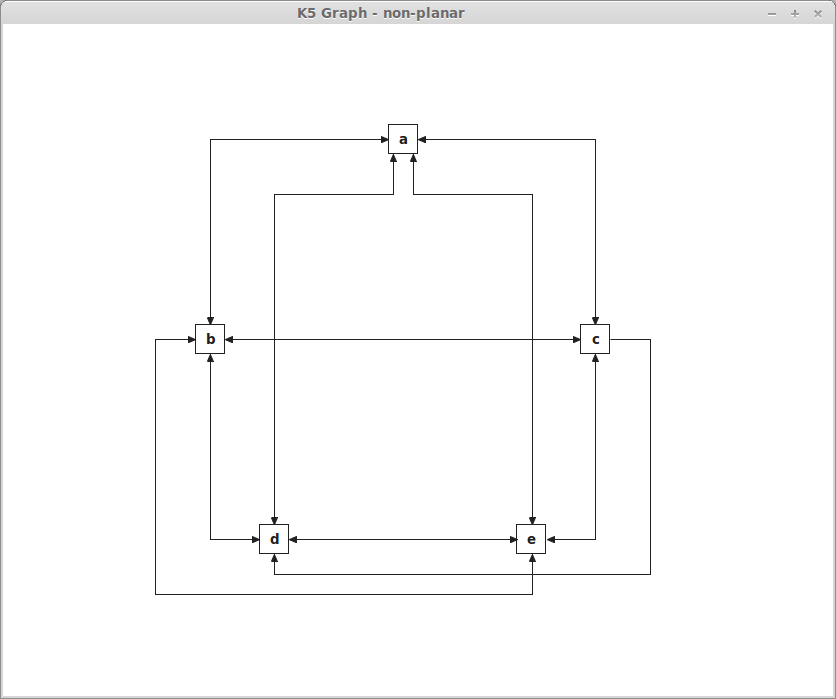
\includegraphics[width=0.65\textwidth]{img/results/k5graph.png}
\caption{The K5 graph. Edges intersect because the graph is not planar. \label{k5}} \end{figure}

\begin{figure}[ht] \centering
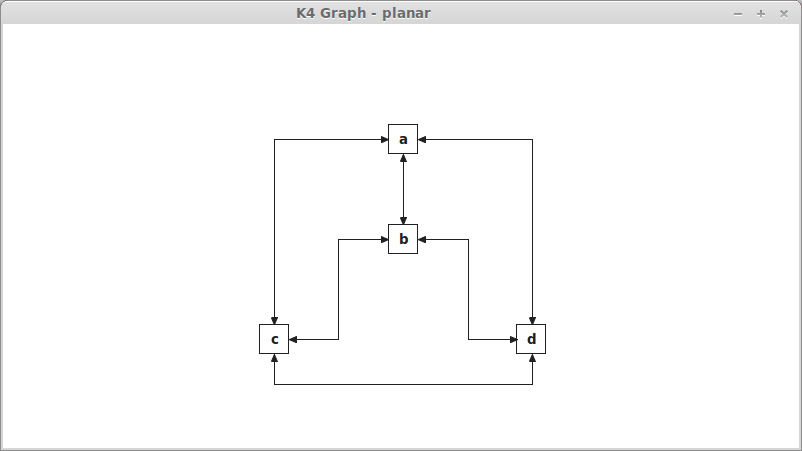
\includegraphics[width=0.75\textwidth]{img/results/k4graph.png}
\caption{The K4 graph. Planarity is preserved. \label{k4}} \end{figure}

\section{Connection routing}

Connection routing is, like planarity testing, an operation which has a relatively low time complexity.
Firstly, it must travesre all edges at least once and ensure that they are connected. Then, all edges which 
are correctly routed are removed from the list and the rest are visited once more. The closest approximation 
for this operation is O($|E| * \log |E|$).

Correctness regarding routing means that all connections are orthogonal. This is done by the router module 
itsefl, because one of the conditions for considering a path correctly routed is it being orthogonal.

\section{Time consumed per module}

Knowing in which module the application spends the majority of the processing time is an important metric 
to analyze for possible optimizations. Since the modules are mainly independent, we can easily time exactly 
how much of the processing time is spent in a certain phase. 

In order to correctly analyze this metric, we shall consider two different cases. In the first one, the input 
graph is not planar, while in the second the graph is planar. In both scenarios, the number of nodes in the 
graph is the same. After running the application multiple times on the same data sets, we obtain the 
following results shown in figures \ref{pie1} and \ref{pie2}: 

\begin{figure}[ht] \centering
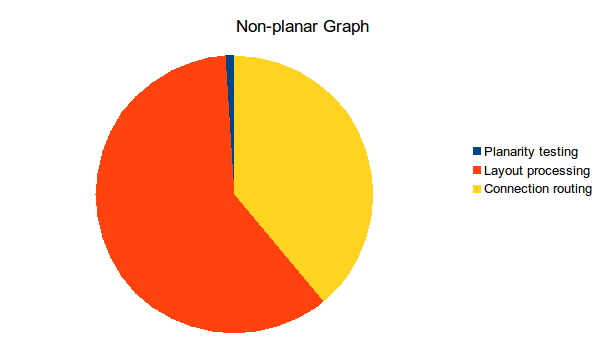
\includegraphics[width=0.65\textwidth]{img/results/nonplanartime.png}
\caption{Timeing results for non-planar graph test \label{pie1}} \end{figure}


\begin{figure}[ht] \centering
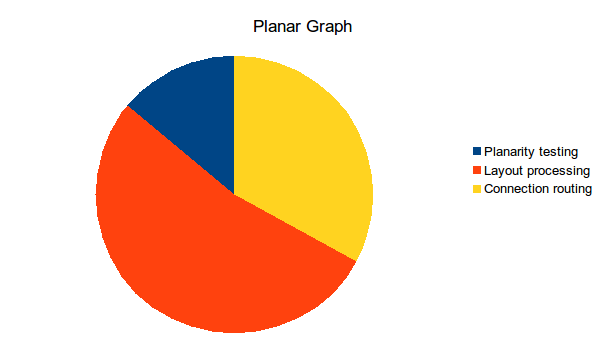
\includegraphics[width=0.65\textwidth]{img/results/planartime.png}
\caption{Timeing results for planar graph test \label{pie2}} \end{figure}

We see that in both cases, the most time is spent in the layout processing module. This result is in 
accordance with our theoretical presumptions: planarity testing is at worst O(${n}$) complexity, and the edge 
routing is proportional with O($|E| * \log |E|$). The complexity of the genetic algorithm surpases both of 
these.

\section{Performance testing}

To see how well the application performs, we must also compare its performance versus that of existing 
implementations. The benchmarks used in these comparative tests are the two implementations mentioned in the 
Related Work chapter: the Graphviz dot command line application and the Eclipse GEF. The benchmarking process 
is performed on tree structured graphs with increasing number of nodes, ranging from 10 to 100000 nodes. We 
analyse only the run time of the computational part of these application, without the GUI enabled.

\begin{figure}[ht] \centering
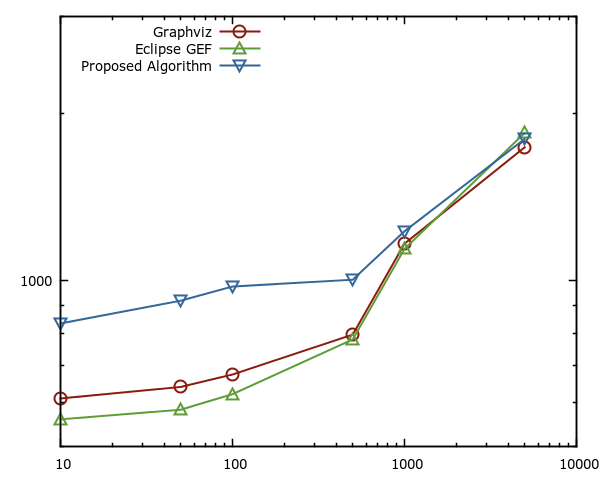
\includegraphics[width=0.65\textwidth]{img/results/under10000.png}
\caption{Performance benchmark for graphs containing under 10000 nodes. Logarithmic scale is used for both X and Y axis \label{chart1}} \end{figure}

\begin{figure}[ht] \centering
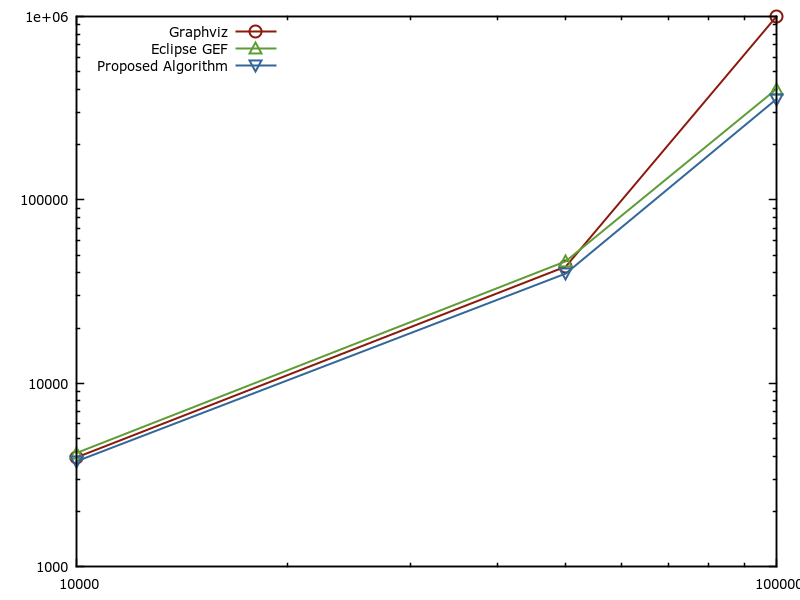
\includegraphics[width=0.65\textwidth]{img/results/over10000.png}
\caption{Performance benchmark for graphs over containing 10000 nodes. Logarithmic scale is used for both X and Y axis \label{chart2}} \end{figure}

The above charts (figures \ref{chart1} and \ref{chart2}) show that for smaller graphs, the all the constraint checking and verifications performed 
by the proposed solution are detrimental to its performance. However, once the number of nodes in the graph starts 
growing, the approximations used and the policy of prefering the local minimum over the global minimum is beneficial.
The point at which the solution becomes favorable is near 10000 nodes.
